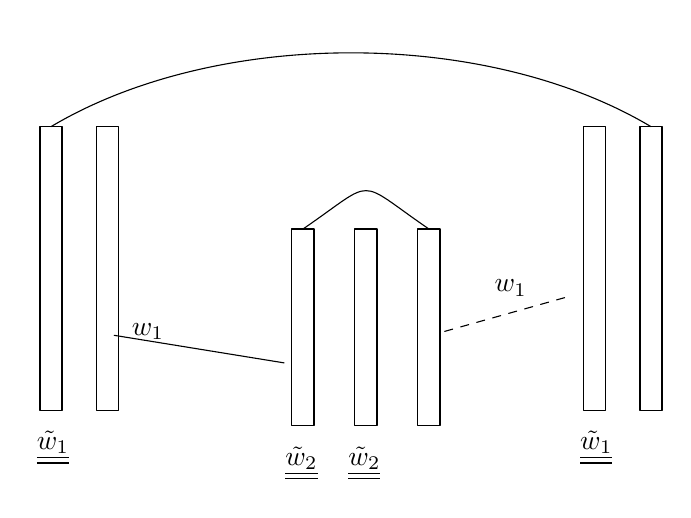
\begin{tikzpicture}[line cap=round,line join=round]

% --- Parameters for consistent sizing ---
\def\W{0.28}   % bar width
\def\H{3.6}    % height of top-level bars
\def\h{2.5}    % height of bottom-level bars
\def\sepT{0.72}  % spacing inside top-level pairs
\def\sepB{0.8}   % spacing between bottom bars

% x-locations of groups
\def\xL{0.0}     % left top pair (first bar at xL)
\def\xB{3.2}     % bottom group (first bar at xB)
\def\xR{6.9}     % right top pair (first bar at xR)

% y baselines
\def\yTop{0.0}   % bottom of top bars
\def\yBot{-0.2}  % bottom of bottom bars

% --- Draw feature "bars" (open rectangles) ---
% Left top pair (two stride-1 convolutions)
\draw (\xL,\yTop) rectangle ++(\W,\H);
\draw (\xL+\sepT,\yTop) rectangle ++(\W,\H);

% Bottom (three bars, center resolution)
\draw (\xB,\yBot) rectangle ++(\W,\h);
\draw (\xB+\sepB,\yBot) rectangle ++(\W,\h);
\draw (\xB+2*\sepB,\yBot) rectangle ++(\W,\h);

% Right top pair (two stride-1 convolutions after upsampling)
\draw (\xR,\yTop) rectangle ++(\W,\H);
\draw (\xR+\sepT,\yTop) rectangle ++(\W,\H);

% --- Connections ---
% Single-line operation (stride > 1): downsampling from top-left to bottom-left
\draw (\xL+0.92*\sepT+\W,0.95) -- (\xB-0.1,0.6);
\node[anchor=west] at (\xL+0.92*\sepT+\W+0.1,1.0) {$w_1$};

% Dashed transpose operation: from bottom-right back to top-right
\draw[dashed] (\xB+2*\sepB+\W+0.06,1.0) -- (\xR-0.16,1.45);
\node[anchor=west] at (\xR-1.25,1.55) {$w_1$};

% Curved skip (copy-and-add) at top level
\draw (\xL+0.5*\W,\yTop+\H) .. controls + (2.1,1.25) and +(-2.1,1.25) ..
      (\xR+\sepT+0.5*\W,\yTop+\H);

% Curved skip (copy-and-add) at bottom level
\draw (\xB+0.5*\W,\yBot+\h) .. controls + (0.95,0.65) and +(-0.95,0.65) ..
      (\xB+2*\sepB+0.5*\W,\yBot+\h);

% --- Labels for stride-1 convolutions (double-underlined weights) ---
\node[anchor=north] at (\xL+0.23*\sepT,\yTop-0.14) {$\underline{\underline{\tilde w_1}}$};
\node[anchor=north] at (\xB+0.12,\yBot-0.14) {$\underline{\underline{\tilde w_2}}$};
\node[anchor=north] at (\xB+\sepB+0.12,\yBot-0.14) {$\underline{\underline{\tilde w_2}}$};
\node[anchor=north] at (\xR+0.23*\sepT,\yTop-0.14) {$\underline{\underline{\tilde w_1}}$};

\end{tikzpicture}